\documentclass[a4paper,
fontsize=11pt,
%headings=small,
oneside,
numbers=noperiodatend,
parskip=half-,
bibliography=totoc,
final
]{scrartcl}

\usepackage[babel]{csquotes}
\usepackage{synttree}
\usepackage{graphicx}
\setkeys{Gin}{width=.4\textwidth} %default pics size

\graphicspath{{./plots/}}
\usepackage[ngerman]{babel}
\usepackage[T1]{fontenc}
%\usepackage{amsmath}
\usepackage[utf8x]{inputenc}
\usepackage [hyphens]{url}
\usepackage{booktabs} 
\usepackage[left=2.4cm,right=2.4cm,top=2.3cm,bottom=2cm,includeheadfoot]{geometry}
\usepackage[labelformat=empty]{caption} % option 'labelformat=empty]' to surpress adding "Abbildung 1:" or "Figure 1" before each caption / use parameter '\captionsetup{labelformat=empty}' instead to change this for just one caption
\usepackage{eurosym}
\usepackage{multirow}
\usepackage[ngerman]{varioref}
\setcapindent{1em}
\renewcommand{\labelitemi}{--}
\usepackage{paralist}
\usepackage{pdfpages}
\usepackage{lscape}
\usepackage{float}
\usepackage{acronym}
\usepackage{eurosym}
\usepackage{longtable,lscape}
\usepackage{mathpazo}
\usepackage[normalem]{ulem} %emphasize weiterhin kursiv
\usepackage[flushmargin,ragged]{footmisc} % left align footnote
\usepackage{ccicons} 
\setcapindent{0pt} % no indentation in captions
\usepackage{xurl} % Breaks URLs

%%%% fancy LIBREAS URL color 
\usepackage{xcolor}
\definecolor{libreas}{RGB}{112,0,0}

\usepackage{listings}

\urlstyle{same}  % don't use monospace font for urls

\usepackage[fleqn]{amsmath}

%adjust fontsize for part

\usepackage{sectsty}
\partfont{\large}

%Das BibTeX-Zeichen mit \BibTeX setzen:
\def\symbol#1{\char #1\relax}
\def\bsl{{\tt\symbol{'134}}}
\def\BibTeX{{\rm B\kern-.05em{\sc i\kern-.025em b}\kern-.08em
    T\kern-.1667em\lower.7ex\hbox{E}\kern-.125emX}}

\usepackage{fancyhdr}
\fancyhf{}
\pagestyle{fancyplain}
\fancyhead[R]{\thepage}

% make sure bookmarks are created eventough sections are not numbered!
% uncommend if sections are numbered (bookmarks created by default)
\makeatletter
\renewcommand\@seccntformat[1]{}
\makeatother

% typo setup
\clubpenalty = 10000
\widowpenalty = 10000
\displaywidowpenalty = 10000

\usepackage{hyperxmp}
\usepackage[colorlinks, linkcolor=black,citecolor=black, urlcolor=libreas,
breaklinks= true,bookmarks=true,bookmarksopen=true]{hyperref}
\usepackage{breakurl}

%meta
%meta

\fancyhead[L]{Redaktion LIBREAS\\ %author
LIBREAS. Library Ideas, 46 (2024). % journal, issue, volume.
\href{https://doi.org/10.18452/31222}{\color{black}https://doi.org/10.18452/31222}
{}} % doi 
\fancyhead[R]{\thepage} %page number
\fancyfoot[L] {\ccLogo \ccAttribution\ \href{https://creativecommons.org/licenses/by/4.0/}{\color{black}Creative Commons BY 4.0}}  %licence
\fancyfoot[R] {ISSN: 1860-7950}

\title{\LARGE{Editorial \#46: Bestandserhaltung in Bibliotheken}}% title
\author{Redaktion LIBREAS} % author

\setcounter{page}{1}

\hypersetup{%
      pdftitle={Editorial \#46: Bestandserhaltung in Bibliotheken},
      pdfauthor={Redaktion LIBREAS},
      pdfsubject={LIBREAS. Library Ideas, 46 (2024)},
      pdfkeywords={Editorial, Bibliothekswesen, Bestandserhaltung},
      pdflicenseurl={https://creativecommons.org/licenses/by/4.0/},
      pdfcopyright={CC BY 4.0 International},
      pdfcontacturl={http://libreas.eu},
      pdfurl={https://doi.org/10.18452/31222},
      pdfdoi={10.18452/31222},
      pdflang={de},
      pdfmetalang={de}
     }



\date{}
\begin{document}

\maketitle
\thispagestyle{fancyplain} 

%abstracts

%body
Jeder Call for Paper ist eine Wette darauf, dass wir ein
Schwerpunktthema gewählt haben, welches viele Kolleg*innen nicht nur
interessiert, sondern auch anspornt, Beiträge zu produzieren. Es ist
immer eine begründete Wette -- die Themen sind jeweils interessant für
uns, die Redaktion, die ja im engeren oder weiteren Sinn im
Bibliothekswesen verankert ist. Oder aber es sind Themen, deren
Bedeutung wir wahrnehmen. Dabei kommen sehr oft sehr interessante,
\enquote{volle} Ausgaben zustande. Die
\href{https://libreas.eu/ausgabe45/inhalt/}{LIBREAS \#45  \enquote{The Sound of
Libraries}} am Anfang 2024 war beispielsweise eine. Aber manchmal
tippen wir auch daneben. Wir hatten -- und haben weiterhin -- den
Eindruck, dass die Bestandserhaltung in der tatsächlichen
bibliothekarischen Arbeit eine viel grössere Bedeutung einnimmt, als in
der Fachliteratur sichtbar ist. Aber dies hat leider nicht viele
Einreichungen erbracht. In den publizierten Einreichungen ist immerhin
sichtbar, dass es sich um einen gegenwärtigen und dynamischen Bereich
der bibliothekarischen Arbeit handelt. Was erhalten wird, wie es
erhalten wird, mit welchen Kooperationseinrichtungen, verändert sich
kontinuierlich.

Wir wissen nie, woran es liegt, dass einige Themen zu vielen und andere
zu wenigen Einreichungen führen. Ist es das Thema? Das Timing der
Ausschreibung des Themas? Oder gibt es einen anderen Grund? Ist es
vielleicht so, dass – verständlicherweise – viele Kolleg*innen das
Gefühl haben, dass die Gesellschaft langsam etwas arg aus den Fugen ist,
die Umwelt sich gegen die Menschen zu wehren beginnt, die Probleme immer
nur zunehmen und die Krisen permanent werden? Werden darob
bibliothekarische Fragen, und dann noch solche zur Bestandserhaltung,
vielleicht sekundär? Im zweiten Halbjahr 2024 überschlugen sich
bekanntlich und leider die schlechten Nachrichten. Damit zurechtzukommen
und nicht in einer medialen Dauerüberforderung zu versinken, ist
vielleicht die Informationskompetenzanforderung der Stunde. Ob sich aus
der Bibliotheksarbeit und Bibliothekswissenschaft Handlungsanleitungen
für die Praxis ableiten lassen, die an dieser Stelle helfen, wäre
möglicherweise ein faszinierendes Thema für eine kommende Aufgabe.

\begin{figure}[H]
\centering
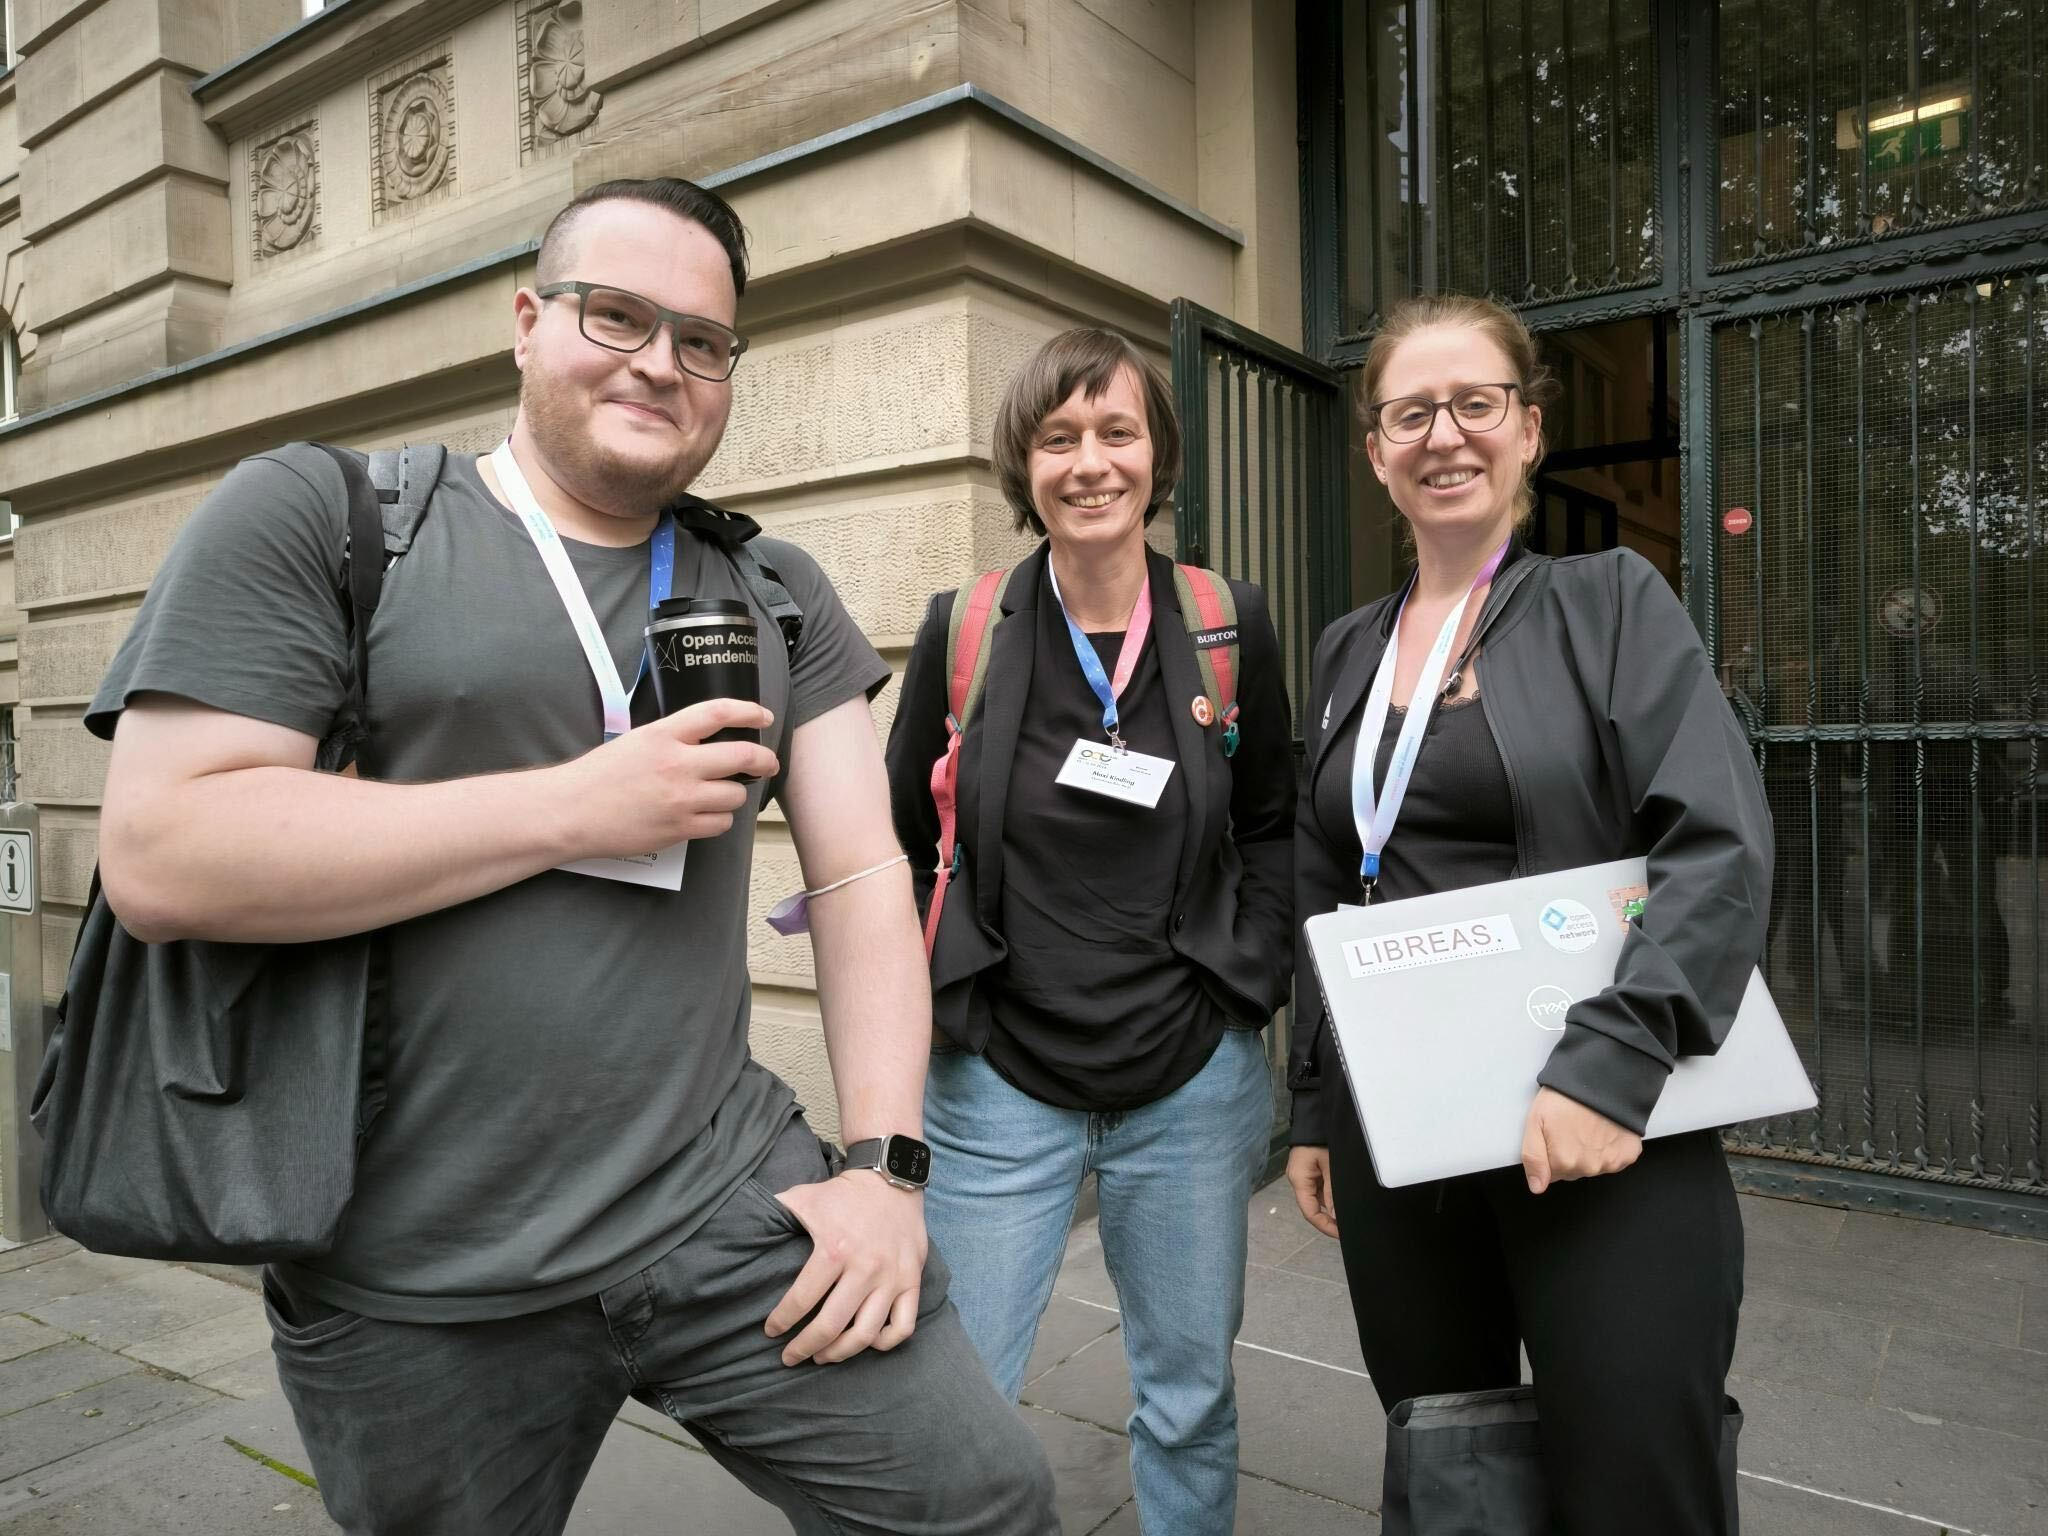
\includegraphics[width=0.5\textwidth]{img/redaktionsorte_koeln_I_Urheber_Andreas_Huebner.jpg}
\caption{Abb. 1: Redaktionsorte XXV: Köln, Herbst 2024 (Foto: Andreas Hübner)}
\end{figure}

\begin{figure}[H]
\centering
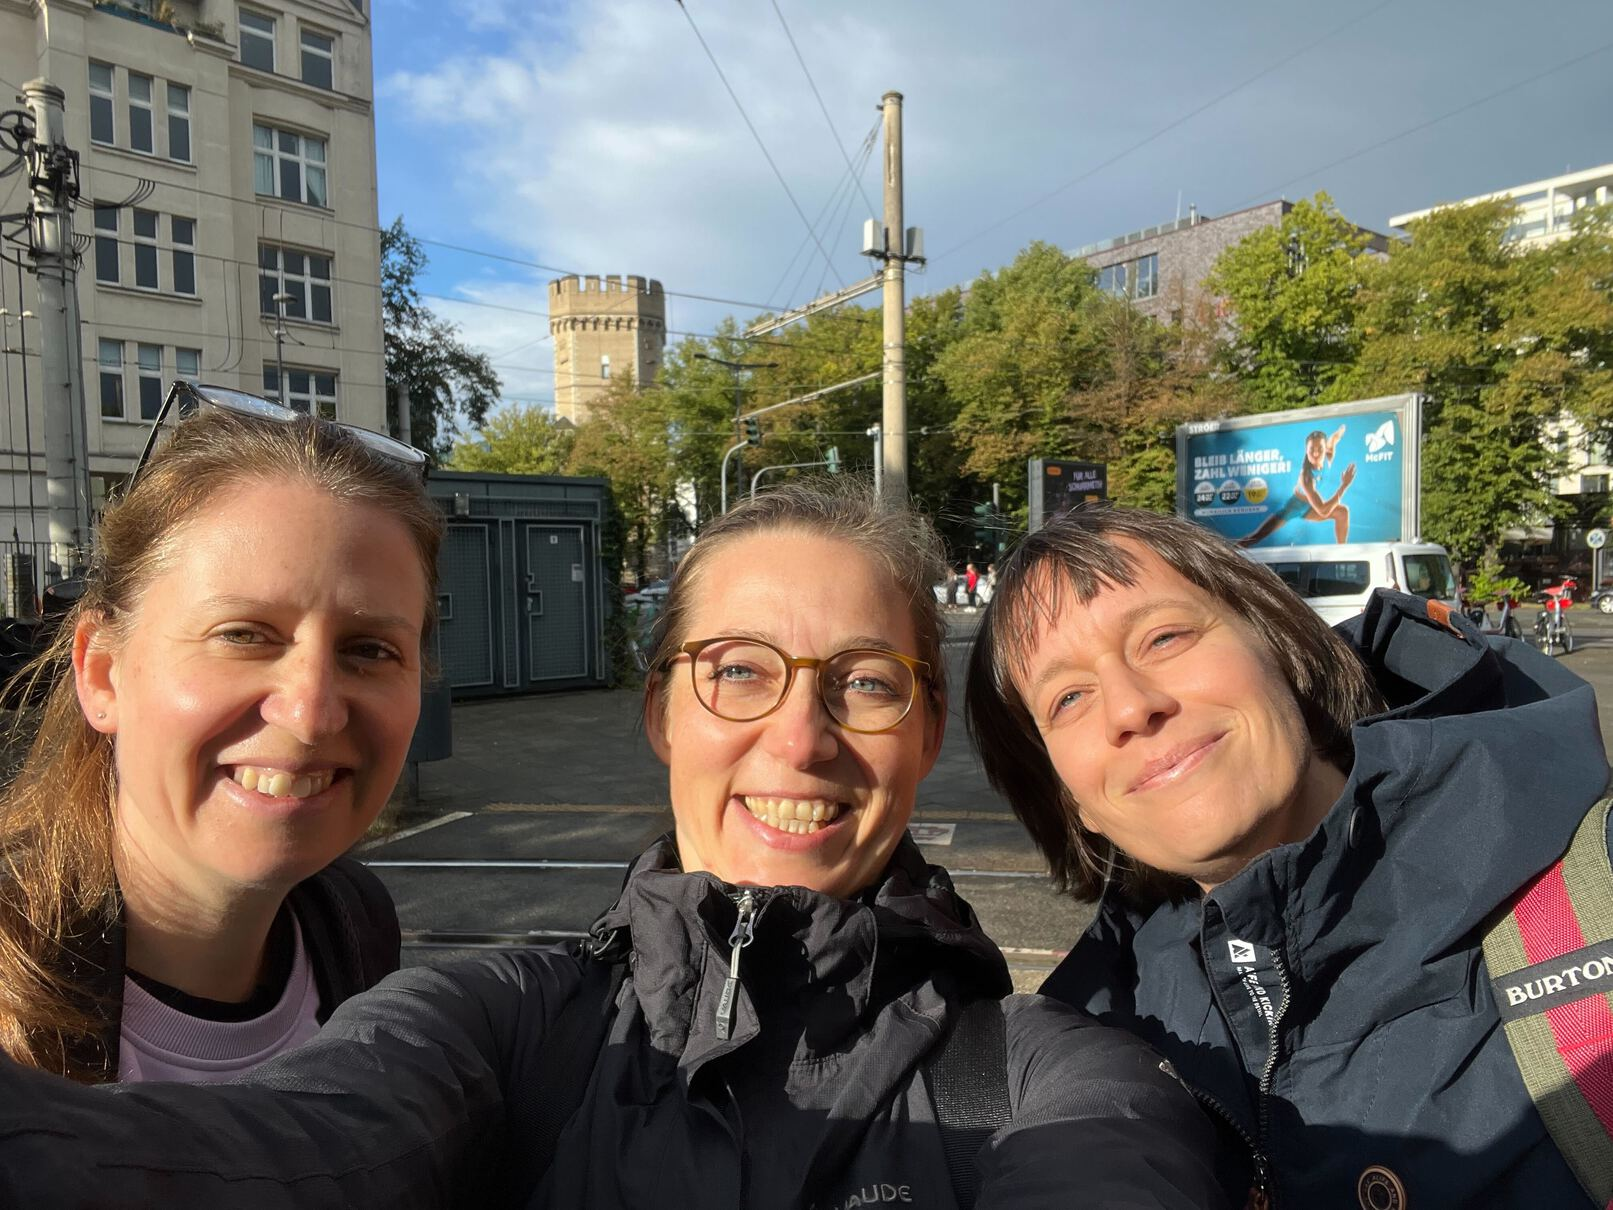
\includegraphics[width=0.5\textwidth]{img/redaktionsorte_koeln_II.jpg}
\caption{Abb. 2: Redaktionsorte XXV: Köln, Herbst 2024}
\end{figure}

So oder so legen wir hiermit die 46. Ausgabe der LIBREAS vor. Damit
nähern wir uns dem 20. Jahr dieser Zeitschrift – was uns sowohl erfreut
als auch erschreckt. So alt fühlen wir uns eigentlich nicht. Zur Feier
dieses Ereignisses werden wir am Freitag vor Pfingsten 2025, dem 6. Juni
2025 nach Berlin zu einer Veranstaltung laden. Wir hoffen, wir sehen
dort – trotz oder gerade wegen allem – viele unserer Leser*innen
persönlich.

Bis dahin,

Ihre / eure Redaktion LIBREAS. Library Ideas

(Berlin, Brandenburg an der Havel, Chur, Göttingen, München)

%autor

\end{document}